\section{Metodología}

La complejidad inherente a este proyecto —que busca conciliar el desarrollo de software productivo con la investigación arquitectónica abstracta— exigió la adopción de un marco metodológico riguroso. Nos basamos en los principios de la \textit{Investigación Basada en Diseño} (\textit{Design Science Research}), un paradigma que permite generar conocimiento científico a través de la construcción y evaluación de artefactos tecnológicos.

Bajo este enfoque, no nos limitamos a la observación pasiva. Actuamos primero como ingenieros pragmáticos para materializar el sistema actual (el artefacto) y posteriormente asumimos el rol de analistas para diseñar su evolución (la teoría). Esta dualidad nos obligó a estructurar el trabajo en tres fases secuenciales y complementarias: la construcción del ecosistema digital, la revisión sistemática de literatura y el modelado de la propuesta arquitectónica.

\subsection{Fase 1: Ingeniería y Construcción del Caso de Estudio}

La materialización del Portal Agro-Comercial no fue un proceso espontáneo, sino el resultado de una planificación deliberada orientada a resolver una necesidad de mercado en el municipio de Teruel.

\subsubsection{Estrategia de Desarrollo Ágil (Scrum)}

Para gestionar la incertidumbre de los requisitos en el sector rural, se adoptó el marco de trabajo \textit{Scrum}. El desarrollo se dividió en cinco \textit{Sprints} de dos semanas cada uno. Esta decisión fue clave: las ceremonias de revisión con los instructores y potenciales usuarios revelaron tempranamente que la rigidez del software era un problema. Cada vez que el cliente (el productor) solicitaba un cambio en el formulario de registro, el equipo debía detener el desarrollo, reempaquetar la aplicación y volver a desplegar, validando empíricamente la necesidad de una arquitectura más flexible.

\subsubsection{Captura de Requisitos y Diseño Centrado en el Usuario (UCD)}

La etapa preliminar se dedicó a comprender el entorno sociotécnico. El levantamiento de la Especificación de Requisitos de Software (SRS) se rigió por una regla innegociable: la accesibilidad. Al caracterizar a nuestro actor principal, se determinó que el nivel de alfabetización digital en el campo es heterogéneo.

Por ello, se diseñaron prototipos de baja fidelidad antes de escribir código, priorizando flujos de navegación lineales. Se definieron roles estrictos (Administrador, Productor, Comprador) y se priorizaron historias de usuario de alto valor, como la ``Carga de Evidencia Fotográfica'' y la ``Gestión de Precios por Unidad de Medida''. Arquitectónicamente, se optó por desacoplar las capas:

\begin{itemize}
    \item \textbf{Capa de Presentación (Frontend):} Desarrollada en \textbf{Angular}, elegida por su robustez en el manejo del estado del cliente y su capacidad de funcionar como SPA (\textit{Single Page Application}), vital para zonas con intermitencia de red.
    \item \textbf{Capa de Negocio y Datos (Backend):} Implementada en \textbf{.NET Core} siguiendo patrones de Arquitectura Limpia (\textit{Clean Architecture}). Esta decisión de usar Inyección de Dependencias fue, sin saberlo en ese momento, la que facilitaría teóricamente la futura inserción de los \textit{Feature Toggles}.
\end{itemize}

\subsubsection{Infraestructura y Pipeline de Despliegue}

Actualmente, la plataforma reside en \textbf{Microsoft Azure}. Sin embargo, el valor ingenieril radica en la automatización del ciclo de vida. Se implementaron pipelines de CI/CD (Integración y Despliegue Continuos) utilizando \textbf{Jenkins}. El código se compila, prueba y empaqueta en contenedores \textbf{Docker}. Este enfoque de contenerización elimina las discrepancias de configuración (``en mi máquina funciona''), pero también evidenció la limitación central de nuestro estudio: el pipeline es monolítico. Para liberar una sola línea de código, se debe reconstruir y redesplegar todo el contenedor, lo que causa tiempos de inactividad.

% --- INICIO FIGURA: Stack Tecnológico ---
\begin{figure}[htbp]
    \centering
    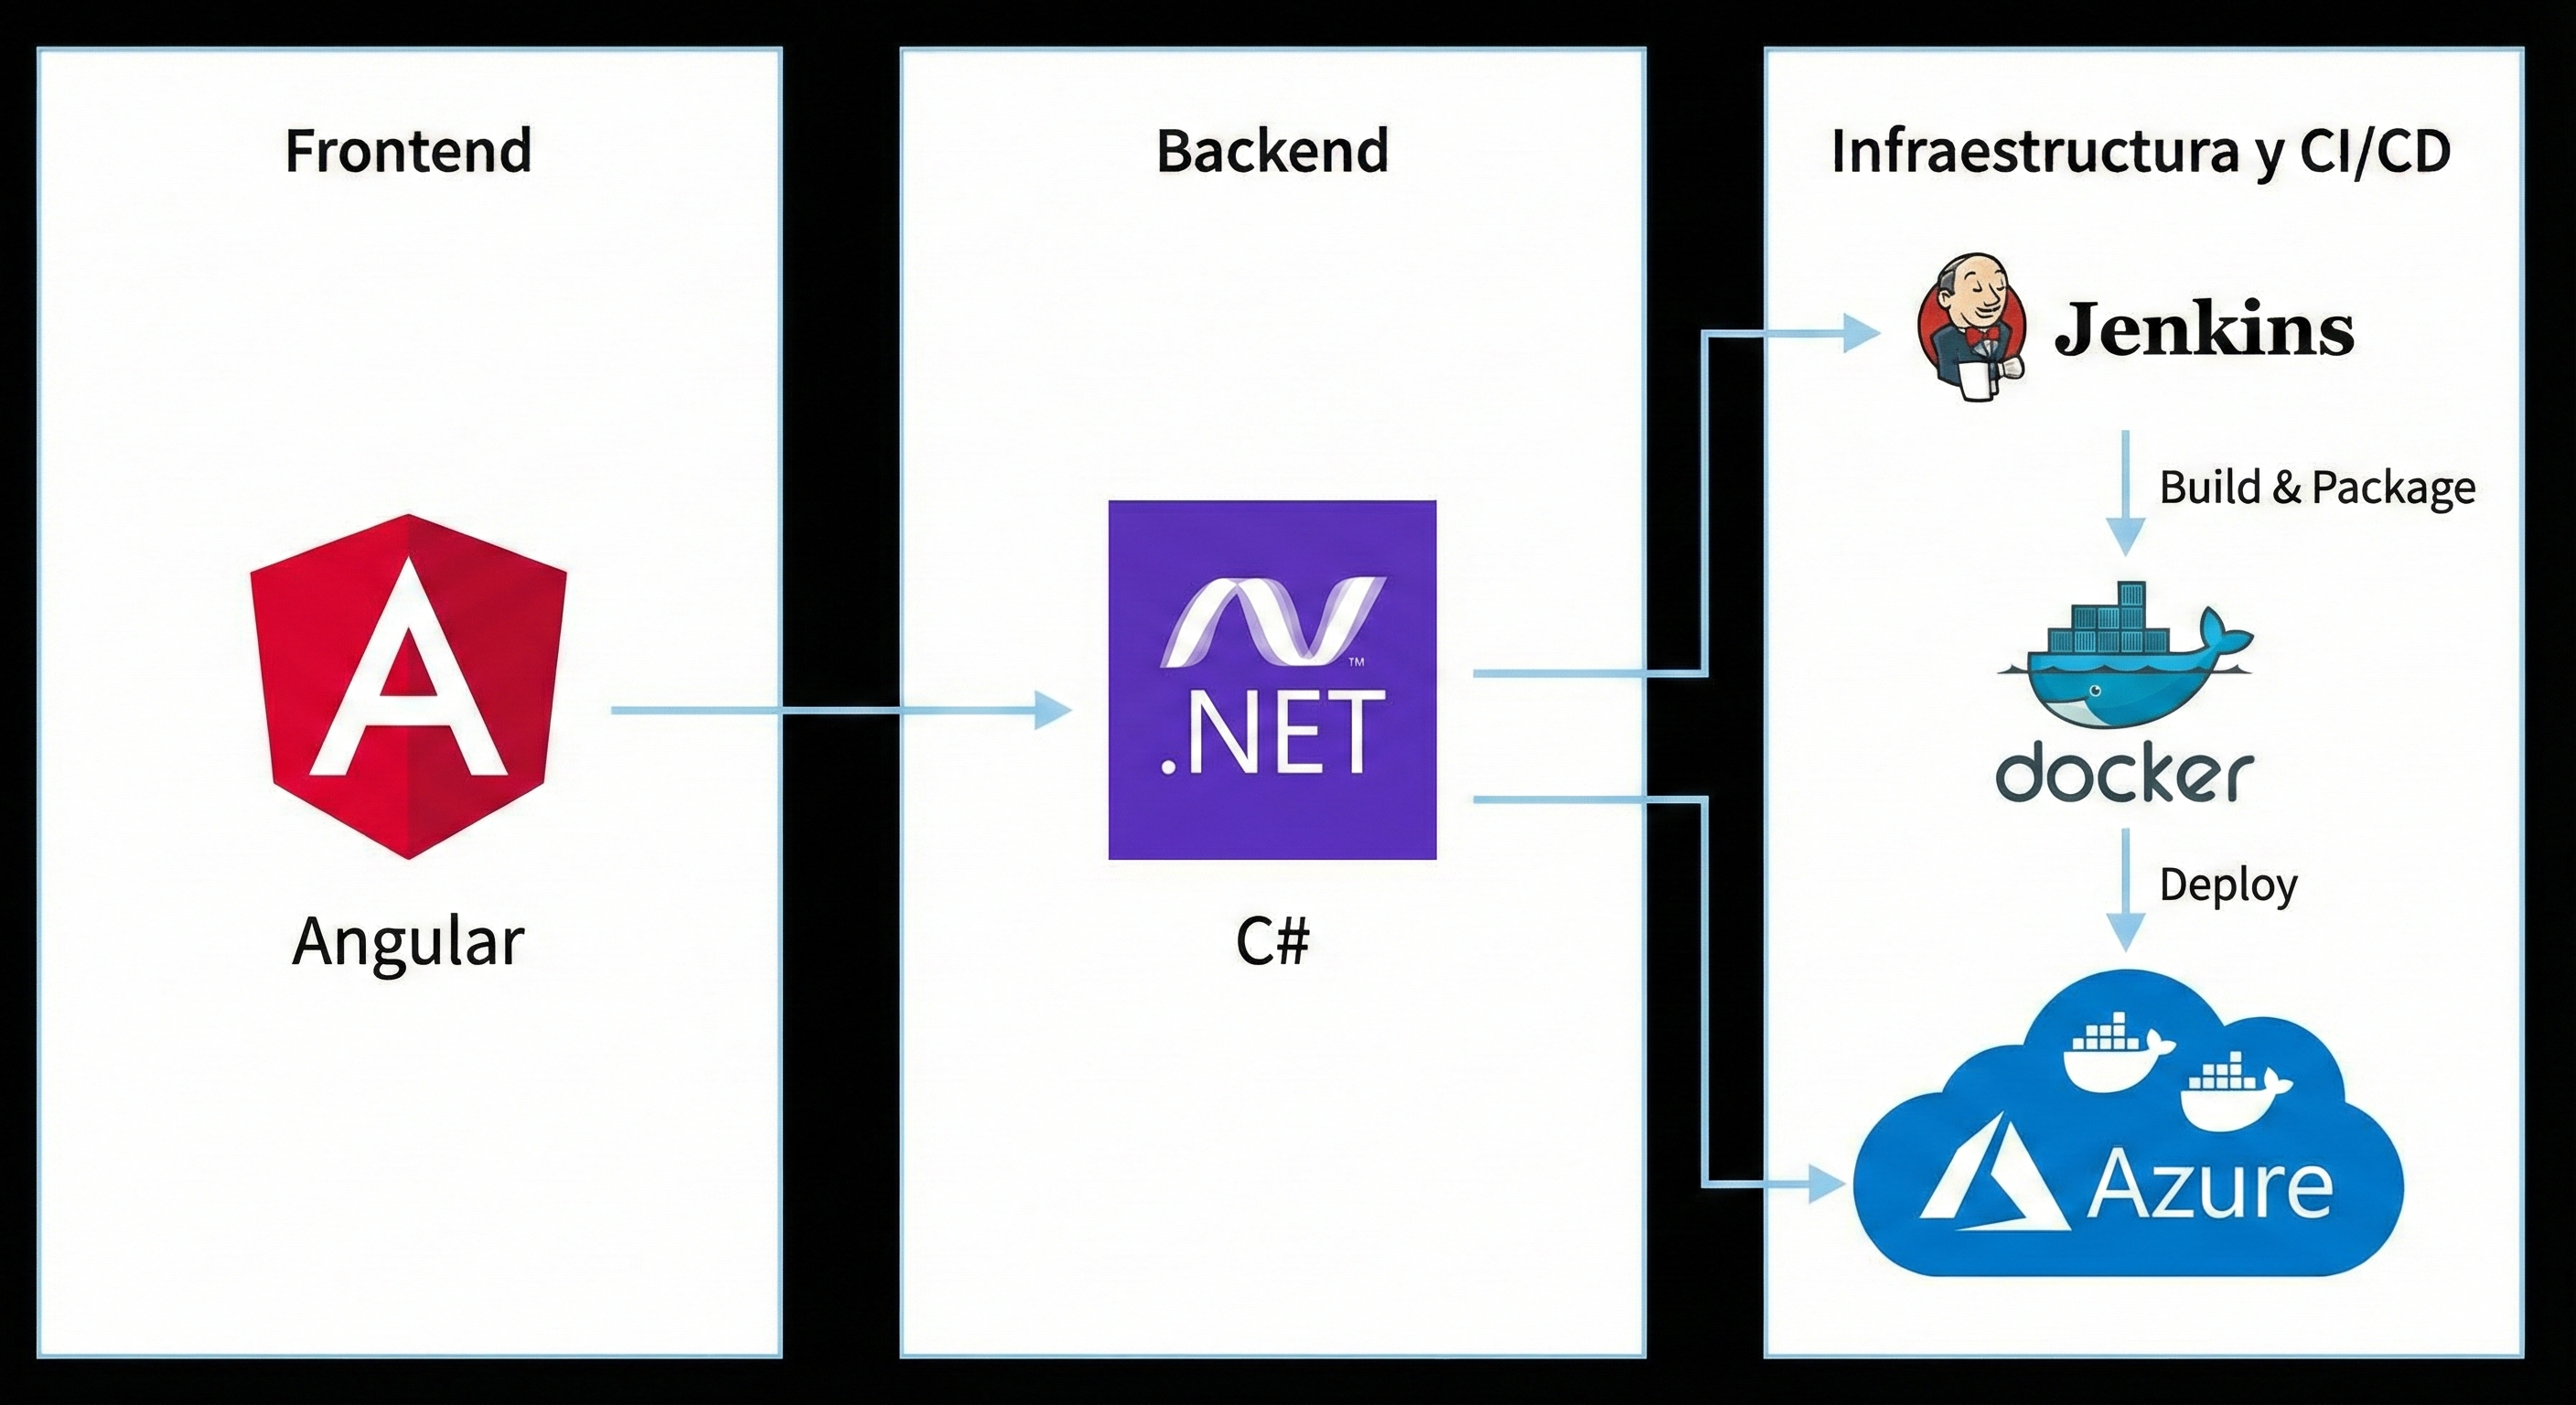
\includegraphics[width=0.9\columnwidth]{graphics/stack_tecnologico.png}
    \caption{Diagrama detallado del stack tecnológico y el flujo de despliegue actual (As-Is). Se observa la linealidad del pipeline en Jenkins que obliga al redespliegue total del contenedor en Azure ante cualquier cambio.}
    \label{fig:stack_tecnologico}
\end{figure}
% --- FIN FIGURA ---

\subsection{Fase 2: Protocolo de Revisión Sistemática}

Dado que el portal no nació con capacidades de configuración dinámica, la segunda fase fue de carácter investigativo. Fue necesario realizar una inmersión profunda en el estado del arte para trazar una ruta segura de adopción de \textit{Feature Toggles}.

\subsubsection{Criterios de Selección y Búsqueda}

Se llevó a cabo una revisión sistemática de literatura cubriendo una ventana de observación de 9 años (2016--2025). Las búsquedas se realizaron en bases de datos indexadas utilizando cadenas como \textit{``Feature Flags AND Technical Debt''} y \textit{``Continuous Delivery in Legacy Systems''}. De un universo inicial de documentos, se filtraron y seleccionaron 20 artículos clave.

El criterio de inclusión fue estricto: no se buscaban textos teóricos genéricos, sino estudios que documentaran:

\begin{enumerate}
    \item \textbf{Transiciones Arquitectónicas:} Cómo pasar de monolito a sistemas dinámicos \cite{meyer2016continuous}.
    \item \textbf{Métricas de Impacto:} Datos cuantitativos sobre complejidad ciclomática \cite{sharma2024complexity}.
    \item \textbf{Gobernanza:} Estrategias para eliminar el código muerto \cite{sridharan2020piranha}.
\end{enumerate}

\subsubsection{Análisis y Taxonomía}

Para estructurar la propuesta, se utilizó la taxonomía de \cite{torres2020differences} como filtro primario. Esto fue crucial para evitar ambigüedades: se distinguió claramente entre una ``Opción de Configuración'' (estática, requiere reinicio) y un verdadero \textit{Feature Toggle} (dinámico, en tiempo de ejecución). Asimismo, se integró la visión de \cite{dupont2022unifying}, quienes proponen ver los toggles no como parches, sino como una evolución de las Líneas de Productos de Software (SPL), lo cual resulta pertinente para la escalabilidad futura del portal a otros municipios.

\subsection{Fase 3: Modelado y Mapeo Arquitectónico}

En la etapa final, se cruzó la realidad del código (Fase 1) con la teoría recolectada (Fase 2). No se procedió a escribir código de manera arbitraria, sino a realizar un \textbf{análisis estático} del repositorio existente.

Siguiendo las heurísticas de detección de \cite{li2020capture} y la propuesta reciente de \cite{wang2025tsdetector}, se identificaron los ``puntos calientes'' (\textit{hotspots}) en los controladores de .NET y los servicios de Angular donde la inyección de condicionales era viable sin romper los principios SOLID.

Finalmente, conscientes del riesgo de degradación del software, se diseñó un protocolo de gobernanza preventiva. Basándonos en el estudio de motivaciones de desarrolladores de \cite{abdalkareem2021removal}, se definieron reglas de ``Definición de Hecho'' (DoD) que incluyen la eliminación obligatoria del toggle, asegurando que la solución propuesta sea sostenible y no se convierta en lo que \cite{ortiz2021toggledebt} denomina un ``cementerio de deuda técnica''.
